Two naturally-occurring isotopes of xenon, \Xe{134} and \Xe{136}, can undergo \bb decay. The latter, with a higher $Q$ value (2458 keV), is preferred for \bbonu decay searches. It constitutes only 8.86\% of natural xenon, but the enrichment process is relatively simple and cheap compared to that of other \bb isotopes. The two-neutrino decay mode of \Xe{136} is slow, $2.2\times10^{21}$~years (see table~\ref{tab:bb2nu_exp}), and hence the experimental requirement for energy resolution is less severe than for other \bb sources. Furthermore, xenon is a suitable detection medium with strong scintillation and ionization primary signals in both its gaseous and liquid phase.

The Milano experiment \cite{Zanotti:1991vh}, running at LNGS in the late 1980s, made use of a multiwire proportional chamber (MWPC) filled with 4.4~kg of xenon gas (enriched to 64\% in \Xe{136}) at a pressure of 9.5 bars. Its detection efficiency was $\sim35\%$, the energy resolution was 4.5\% FWHM at 2.5~MeV and the background rate in the energy region of interest was 11~\ckky. After accumulating almost 2 kg~yr of exposure, the experiment set a lower limit to the half-life of \Xe{136} of $2.0\times10^{22}$~years (90\% CL).

The Gotthard TPC \cite{Luscher:1998sd, Vuilleumier:1993zm} operated at the St.\ Gotthard road tunnel, Switzerland, in the 1990s. The detector was filled at a pressure of 5~atm with a 96:4 mixture of enriched xenon gas and methane; the active volume of the detector, of about 180 litres, contained 3.3~kg of \Xe{136}. The TPC was read out with a MWPC located at the anode. The key idea of the experiment was the use of the tracking capabilities of the TPC to discriminate between signal and background events using their energy deposition pattern ($\mathrm{d}E/\mathrm{d}x$), achieving a background rejection efficiency above 98\% and a background rate in the region of interest of about 0.01 \ckkbby. The measured energy resolution, 6.5\% FWHM at 2500 keV, was rather modest for xenon. The following limit to the  \bbonu-decay half-life was reported: $\Tonu > 4.4\times10^{23}$~years at 90\% CL. 

More recently, the Enriched Xenon Observatory (EXO) searched for \bbonu\ using a cylindrical TPC, EXO-200, filled with about 110~kg of liquid xenon (LXe) enriched to 80.6\% in \Xe{136} \cite{EXO-200:2019rkq}. The TPC consisted of two drift regions, each with a radius of 18~cm and a drift length of 20~cm, separated by a central cathode. Energy depositions in LXe produce both scintillation light and ionization. In EXO-200, the ionization charge was read out at each anode by crossed-wire planes, while the scintillation light was collected by arrays of avalanche photodiodes (APDs) located behind the wire planes. The total energy deposited was determined from the combination of the charge and light signals. The TPC was housed in a thin-walled copper vessel, and surrounded by several layers of passive and active shielding, including 50~cm of cryofluid and 25~cm of lead. A plastic scintillator muon veto surrounded the experiment on four sides. The detector operated at the Waste Isolation Pilot Plant (WIPP), in New Mexico, United Stated. The signal detection efficiency was above 96\%, the energy resolution at the $Q$ value of \Xe{136} was 2.7\% FWHM, and the measured background rate in the ROI was approximately $2\times10^{-3}$~keV$^{-1}$~kg$^{-1}$~yr$^{-1}$. After accumulating a total exposure of 234.1~kg~yr, EXO-200 set a lower limit on the \bbonu\ half-life of \Xe{136} of $3.5\times10^{25}$~years at 90\% CL.

\begin{figure}[t!b!]
\begin{center}
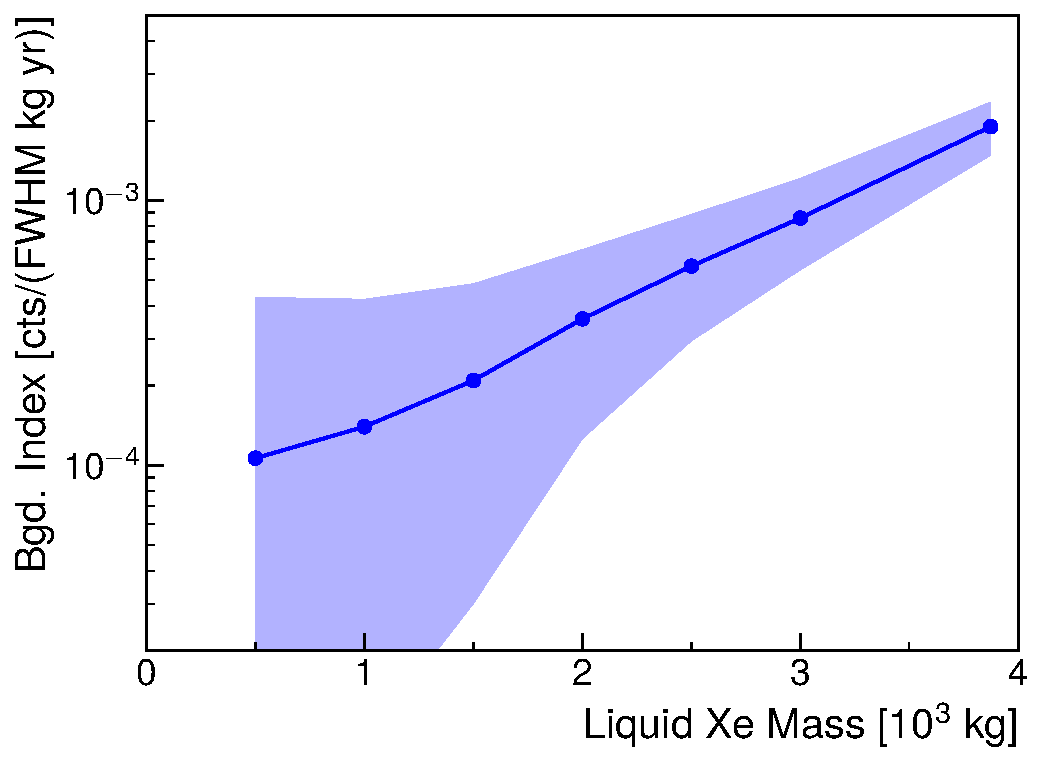
\includegraphics[width=0.75\textwidth]{img/nexo}
%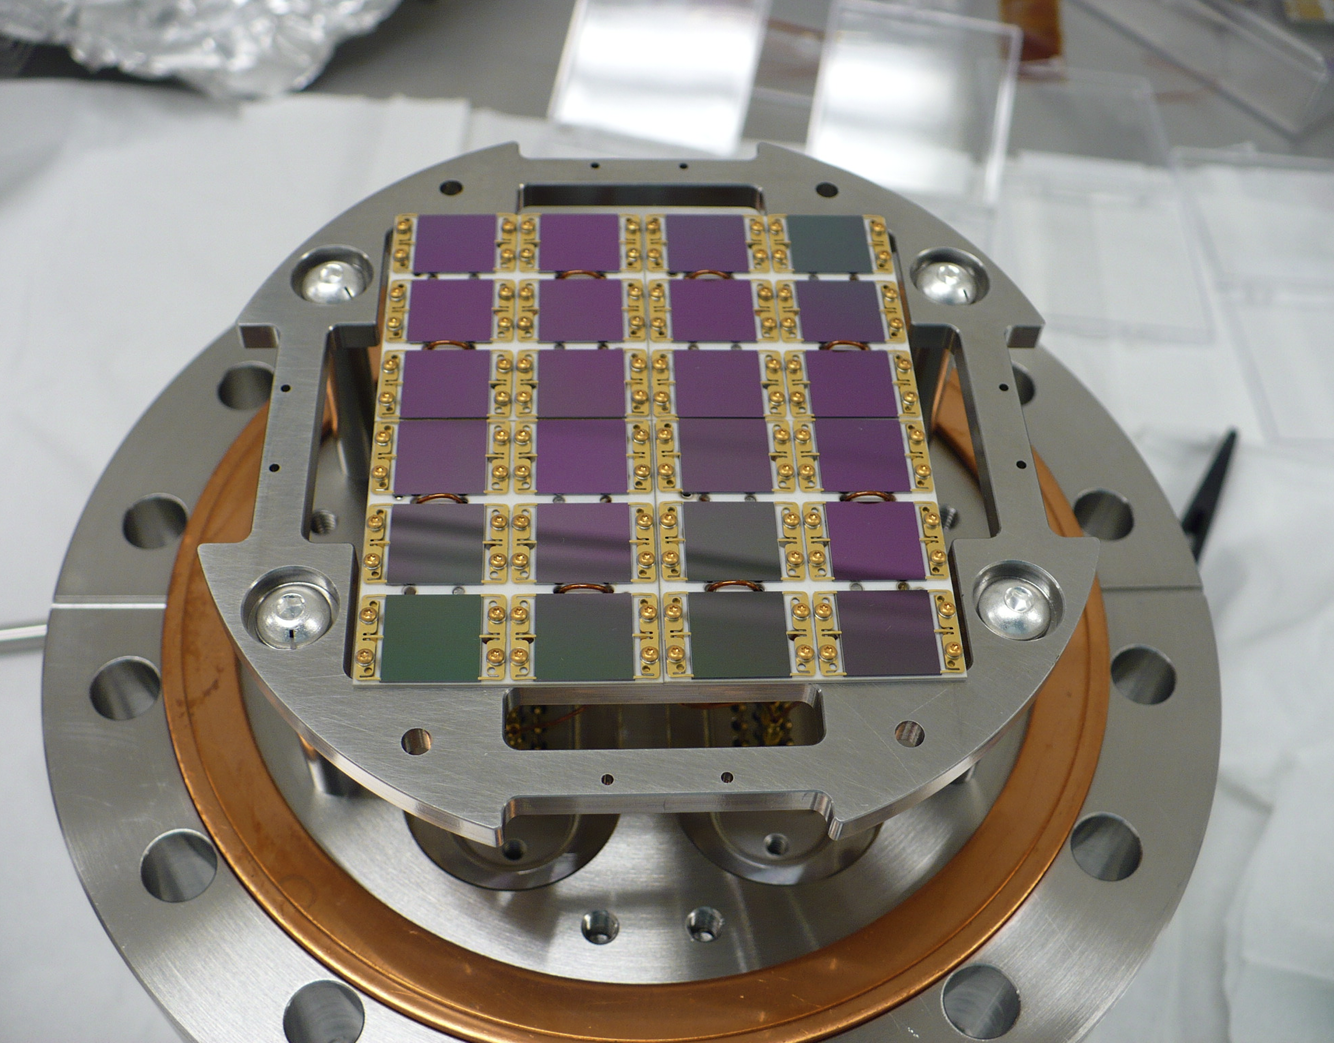
\includegraphics[width=0.475\textwidth]{img/nexo_sipms}
\end{center}
\caption{Expected background index (nEXO simulation) as a function of the active mass of LXe. The plot illustrates the tradeoff in self-shielding calorimeters between background reduction and active mass. } \label{fig:nexo}
\end{figure}

nEXO \cite{nEXO:2018ylp,nEXO:2021ujk}, a follow-on to EXO-200, is a proposed next-generation \bbonu\ experiment with a LXe TPC of 5000~kg of isotopically enriched xenon. It will consist of a single-drift cylindrical TPC 113~cm in diameter and 118~cm in length, holding an active mass of xenon close to 3650~kg. Charge will be collected at the anode with long crossed electrode strips, while a barrel of VUV-sensitive silicon photomultipliers (SiPMs) surrounding the active volume will detect the LXe scintillation light. The TPC vessel, made of copper, will be surrounded by 33~tons of cryogenic fluid, which serves as both thermal bath and radiation shield. nEXO plans to reduce the background rate achieved in EXO-200 to $7\times10^{-5}~\mathrm{counts/(FWHM\cdot kg\cdot yr)}$ taking advantage of the relatively short attenuation length in LXe of $\gamma$ rays of 2.5~MeV, about 8.7~cm, selecting only events occurring in the innermost 2000~kg of the TPC (see fig. \ref{fig:nexo}). The expected energy resolution of the detector is 1.9\% FWHM at 2.5~MeV. This performance results in a projected half-life sensitivity of $1.35\times10^{28}$~years at 90\%CL.
  
  \begin{figure}[t!b!]
\begin{center}
\includegraphics[width=0.95\textwidth]{img/nextTracks.pdf}
%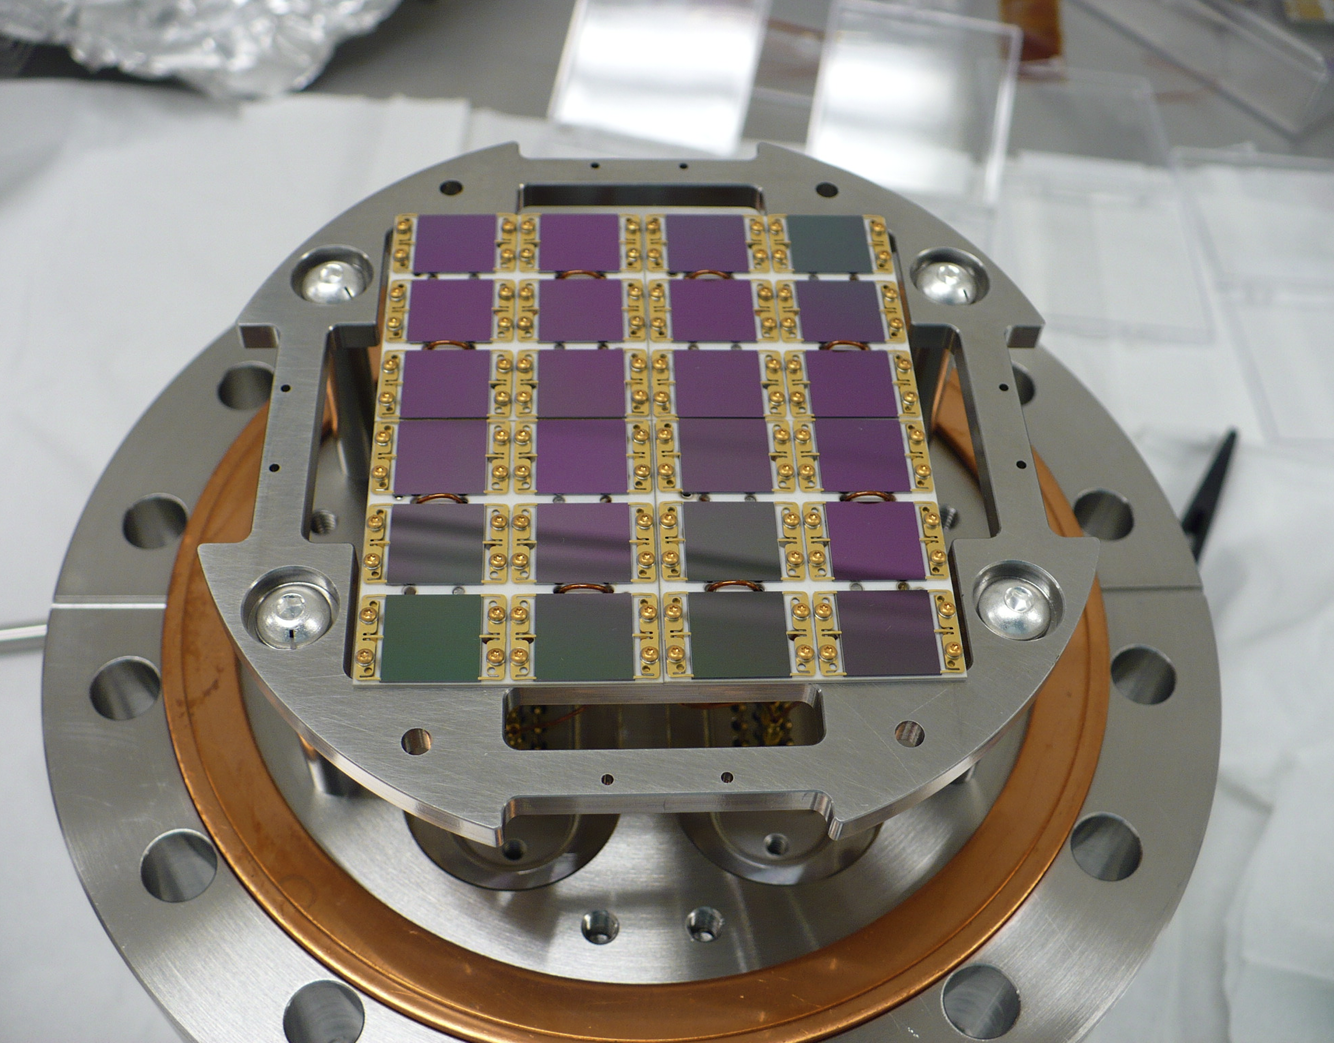
\includegraphics[width=0.475\textwidth]{img/nexo_sipms}
\end{center}
\caption{Reconstruction of the trajectories of double electrons (upper row) and single electrons (lower row) produced at  the Th double escape peak, with energies of 1.6 MeV, recorded in NEXT-White data. Two-electrons deposit energy at the end of each extrema of the track, while single electrons are characterized by a single energy blob. This feature provides a reduction in the background rate of almost two orders of magnitude.} \label{fig:next}
\end{figure}
  
  
NEXT \cite{NEXT:2015wlq, NEXT:2020amj} is an international effort dedicated to the search for \bbonu\ decay in \Xe{136} using high-pressure xenon gas time projection chambers (HPXeTPC) with amplification of the ionization signal by electroluminescence (EL). This detector technology takes advantage of the inherently low fluctuations in the production of ionization pairs (i.e., small Fano factor) in xenon gas to achieve an energy resolution better than 1\% FWHM at \Qbb, significantly better than that of other \Xe{136}-based double-beta decay experiments \cite{Nygren:2009zz}. Moreover, the tracks left in gaseous xenon by \bbonu\ events have distinct features that can be used for background rejection ((see fig. \ref{fig:nexo}). Over the last decade, the NEXT Collaboration has proven the performance of the HPXeTPC technology in the key parameters required for the observation of \bbonu\ decay. with the underground operation at the Laboratorio Subterráneo de Canfranc of NEXT-{\sc White}, an asymmetric, radiopure HPXeTPC containing approximately 5~kg of xenon at 10~bar pressure. 
The NEXT-100 detector, scheduled to start operation in 2023, constitutes the next phase of the program. It is an asymmetric HPXeTPC containing about 100~kg of xenon (enriched at $\sim$90\% in \Xe{136}) at 15~bar. NEXT-100 will reach a sensitivity of about $6\times10^{25}$~year after a run of 3 effective years, for a predicted background rate of at most $4\times10^{-4}$ \ckky. A scaled-up version of this technology, dubbed NEXT-HD, with about 1 tonne of enriched xenon could reach in less than 5 years of operation a sensitivity to the half-life of \bbonu\ decay better than $10^{27}$~years, improving the current limits by at least one order of magnitude. 

Xenon TPCs can, potentially detect (``tag"), the daughter $Ba^{2+}$ cation emitted in the \bbonu\ decay of \Xe{136}, in (delayed) coincidence with the two beta electrons. 
The possibility of barium tagging in a xenon TPC was proposed in 1991\cite{Moe:1991ik} and relied in Ba$^+$ fluorescence imaging using two atomic excitation levels in very low density gas. Recently
the nEXO collaboration has demonstrated the imaging and counting of individual barium atoms in solid xenon by scanning a focused laser across a solid xenon matrix deposited on a sapphire window \cite{Chambers:2018srx}. This is a promising step for barium tagging in liquid xenon, where recombination is frequent and the barium daughters are distributed across charge states from 0 to 2$^+$ \cite{PhysRevC.92.045504}, with sizeable populations of neutral Ba and  Ba$^+$.  

In high pressure gas phase, on the other hand, recombination is minimal \cite{1997NIMPA.396..360B}, and $Ba^{2+}$ dominates. However, in 2015, a promising technique to detect $Ba^{2+}$ in a HPXe, using a layer of molecular indicators was
proposed \cite{Nygren_2015}. The concept that was further developed in \cite{Jones:2016qiq} and spanned a vigorous R\&D program within the NEXT collaboration \cite{McDonald:2017izm,Rivilla:2020cvm}. 
Daughter ion tagging is undoubtedly very challenging from the technical point of view, but the payoff ---the potential to operate in the ``background free'' limit--- for future \bbonu\ experiments aiming at sensitivities of $10^{28}$ year and beyond  would be huge.